\chapter{Indledning}
\label{chap:indledning}

%INTRODUKTION TIL HELE KAPITLET
Indledningsmæssigt starter vi med at beskrive et initierende problem, der omhandler madspild i husstande i Danmark. Her dokumenteres et overordnet og bredt problem. Dette problem skal senere skæres ned til et mere begrænset og specifikt problem.

Herefter introduceres læseren for forbrugerne, altså danskerne i de danske husstande, og de problemer, de muligvis har mht. madlavningen i husstanden. Vi arbejder sammen med to informanter (Merete \& Keld), der begge bor i Aalborg omegn og sørger for madlavningen for deres familier. Informanterne står til rådighed, når vi har spørgsmål vedrørende \fx madlavnings- og madspildsområdet. Disse områder betegner vi som problemområdet. Derudover bruger vi deres hjælp til afprøvning af vores idéer. De hjælper vores udviklingsproces ved at komme med deres meninger om en given idé og forslag til forbedringer.

Ydermere beskrives selve udviklingsopgaven, som vi skal arbejde med og udvikle en løsning til. Hertil bliver informanterne brugt i høj grad ved at give os respons på vores idéer. Vi tager deres idéer i betragtning, når vi skal definere og afgrænse problemet vha. en systemdefinition (beskrivelse af en IT-løsning, udtrykt i naturligt sprog).

\section{Initierende problem}
\label{sec:initierendeproblem}

I Danmark findes der omkring 2,6 millioner husstande \cite{husstande}, der dagligt skal få madlavningen til at gå op i en højere enhed. Der er nemlig mange ting at tage højde for under madlavningen. Der skal tænkes på sundhed for den enkelte, i form af selve kosten, men også sundhed for alle på længere sigt, hvilket opnås ved, at vi i samlet flok skåner miljøet.
En ensformig kost er langt fra lige så sund som en varieret kost. En årsag til ensformighed i madlavningen kan være en travl hverdag, hvor man knytter sig til faste vaner som \fx at lave den samme ret ofte, fordi man synes, den smager rigtig godt og samtidig er lynhurtig at lave. Kosten kan også blive ensformig, fordi man benytter resterne fra madlavningen i nøjagtig samme opskrift dagen efter.
Under madlavningen kan miljøet skånes ved at undgå at smide for meget mad væk. En parcelhusejer smider i gennemsnit 42 kilo spiseligt mad ud om året. \cite{madspildpol} Hvis man ikke vil benytte resterne fra madlavningen i samme opskrift dagen efter, så kan det være svært at finde en ny opskrift at benytte resterne i. I kogebøger bliver det hurtigt uoverskueligt, gang på gang, at blive mødt af opskrifter, der alle kræver en tur i supermarkedet for at få fat på den selleri, man aldrig har. Når man endelig får bevæget sig ned i supermarkedet, så sælges alt i kæmpe portioner. Hakket oksekød findes typisk i pakker med 500 gram som det mindste. Til en enkelt person er dette ofte for meget, og derved risikerer man enten at stå med 100-200 gram hakket oksekød til skraldespanden, eller et problem med hvor dette kød nu skal benyttes. Det er dog muligt at opdele disse store pakker i mindre portioner og fryse dem ned til en anden aften, men tallene for madspild viser, at mange husstande smider meget mad ud, hvilket kan betyde, at de store portioner ikke bliver opdelt i mindre portioner, men blot bliver brugt i madlavningen som de er.

Tal fra Politiken viser, at en parcelhusejer i gennemsnit smider 42 kilo spiseligt mad ud om året. \cite{madspildpol}
Sådanne typer madspild koster desuden danske husholdninger 16 milliarder kroner om året, eller ca. 20 \% af madforbruget af en gennemsnitlig dansk børnefamilie. \cite{madspild16}

\section{Introduktion af forbrugeren}
%Situation

%Formålet med møde 1 er at opnå en større indsigt i informantens mad- og indkøbsvaner og på den måde få en forståelse for hvilke problemer der er mulighed for at løse ved udviklingen af et system.

%Det er på baggrund af møde 1 er det blevet gjort klart, at der blandt informanterne findes flere forskellige problemer vedrørende madlavning, hvoraf nogle er prioriterede højere end andre blandt informanterne. Ved at bruge BATOFF-modellen, er 2 systemdefinitioner blevet lavet. Systemdefinitionerne beskriver kort 2 forskellige systemer, der hver især løser nogle af de, af informanterne, rejste problemstillinger.

\section{Udviklingsopgaven}
\label{sec:udviklingsopaven}

%introduktion
Det primære formål med samtalerne med informanterne er at undersøge, hvordan en almindelig hverdag med madlavning foregår i danske husstande. Ud fra sådan en undersøgelse vil vi være i stand til at forstå, hvordan et system vil være i stand til at hjælpe familierne med madlavningen. Derudover er samtalerne blevet brugt til idégenerering undervejs, da informanterne har nogle gode løsningsidéer, som vi kan arbejde videre med i projektet. 

%opgaven
Vi har nu fået en indsigt i, hvordan de to familier håndterer og planlægger madlavningen i deres travle hverdage. Det kan meget hurtigt blive rutinepræget mad, der bliver serveret, fordi den madansvarlige har kendskab til retten og ved hvor lang tid, der skal bruges på den. Familierne prøver så vidt muligt at bruge så lidt tid på madlavningen som muligt, så de har mere tid til at hygge sig med familien. Det forekommer ofte, at der er madrester fra aftensmaden, og familierne gør deres bedste for at få spist eller genbrugt alle resterne. Dette lykkedes dog ikke hver aften, og derfor bliver der en gang i mellem smidt mad ud i affaldet. 

Når der er madrester fra gårsdagens aftensmad, så har den madansvarlige i familien sjældent tid til manuelt at kigge kogebøger eller hjemmesider med opskrifter igennem for at finde en ret, hvor madresterne kan genbruges. Dette medfører tit, at aftensmaden bliver ensformig og ofte er det blot den samme ret, der bliver genbrugt. På denne måde sparer familierne også tid på madlavningen.

Udviklingsopgaven lyder på, at vi skal udvikle et system, der hurtigt og nemt kan bruges til at planlægge madlavningen i danske husstande. 

%afslutning
Hvordan udføres denne opgave? Vi starter med at formulere systemdefinitioner, der har til formål at løse problemerne mht. planlægningen og madlavningen. Disse systemdefinitioner bliver udarbejdet ud fra de samtaler, vi har haft med informanterne. Derefter præsenterer vi definitioner for informanter, der skal give os deres meninger og idéer vedrørende systemdefinitionerne.
\chapter{Systemvalg}
\label{chap:systemvalg}
%introduktion. formål, metoder -> resultat

\section{Beskrivelse af situationen}
\label{sec:situation}

%indledning
To familier kan ikke repræsentere en befolknings madvaner eller madlavningspolitik. Vi er helt klare over, at vores to informanters madvaner ikke kan generaliseres til hele Danmark. Vi vurderer dog, at samtalerne med informanterne giver et godt billede af, hvordan stituationen, mht. madlavningen og madvaner, ser ud i nogle danske husstande. Merete og Keld kommer fra to forskellige familier i Aalborg.

%situation
Situation er, at begge vore informanter står for madlavningen i deres husstande. De er begge opmærksomme på, at der er dele af aftensmaden, der bliver smidt ud. Denne madspild forekommer selvom, de prøver at genbruge madresterne ved bl.a. at fryse madresterne ned eller genbruge dem den kommende dag i \fx biksemad, supper osv. Det forekommer ofte, at familierne får gårsdagens rester til dagens aftensmad.

%madvaner og madlavning
Det er vigtigt at være opmærksom på, at Merete har været vant til at lave aftensmad til to drenge og en pige ud over hende selv og hendes mand. Ægteparrets børn er flyttet hjemmefra, og de spiser derfor sjældent med hos forældrene. Det er svært at få mængden af aftensmad til at passe, så der ikke er nogen rester, når alle er mætte. Merete er også meget opmærksom på holdbarhedsdatoerne på de forskellige madvarer. Hvis den dato bliver overskredet, så bliver maden smidt ud med det samme.

Derudover forklarer Keld, at han med vilje laver ekstra store portioner til aftensmaden, så familien kan få resterne fra dagens aftensmad den næste dag. Denne strategi benytter Keld sig af, fordi han mener, at der ikke altid er meget tid tilovers til madlavningen. Ægteparret har to små børn, der skal passes og bruges tid på. Ud over at tage sig af børnene, så har de også hver deres arbejde, som skal ses til. Derfor er tid ikke noget, som ægteparret har meget af, og de bruger lignende tricks til at bruge mindre tid på madlavningen og mere tid på at være sammen. Det er helt tydeligt, at tiden er en vigtig faktor for Kelds familie, og det er netop derfor, at familien ofte får de samme retter til aftensmad.

%indkøbsliste
Når det kommer til indkøb af madvarer, så er det ikke altid, at der bliver brugt en indkøbsseddel til at planlægge indkøbet. Den person, der har tid, handler ind. Merete og hendes mand kan bedst lide at gå på opdagelse i supermarkedet, og se om de kan finde nogle gode tilbud, som de kan lave noget aftensmad ud af. Keld derimod står altid for indkøb, og han har ofte en plan i hovedet eller en liste i hånden over, hvad han skal have købt med hjem til aftensmaden. Han påpeger, at det ofte forekommer, at han får købt lidt andet godt (slik osv.) med hjem end der stod på indkøbssedlen.

%madplan
Hverken Merete eller Keld benytter sig af en madplan, når ugens aftensmad skal planlægges. De har ofte idéerne til aftensmaden i hovedet, og madlavningen er rutinepræget. Aftensmaden er meget ensformig, fordi fremgangsmåden er velkendt og derved nem og hurtig at lave. Derudover er det svært for familierne at planlægge tidspunktet for aftensmaden, fordi de alle har jobs, der skal ses til. Derfor ændrer deres planer sig pludseligt, og det vil være svært at styre en madplan, når arbejdstiderne kan variere.

\begin{figure}
\centering
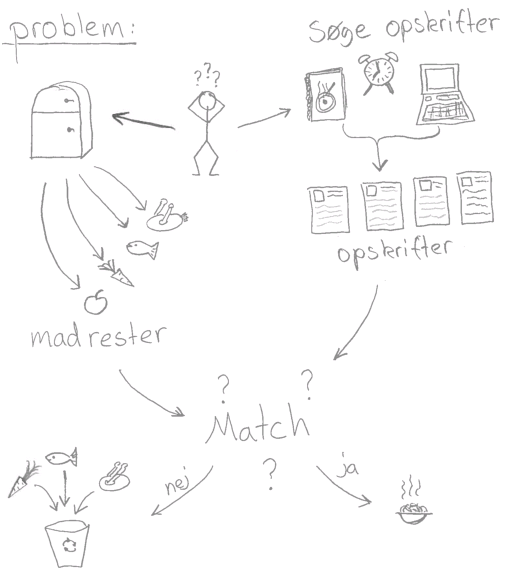
\includegraphics[scale=0.6]{billeder/rigebilleder/problemomraade.png}
\capt{Rigt billede, der visualiserer problemet ved at skulle genbruge madrester.}
\label{fig:rigbillede1}
\end{figure}

Det rige billede i \figref{fig:rigbillede1} viser en bruger, der ikke har tid eller ressourcer til at finde ud af, hvordan madresterne, der er i køleskabet, kan blive brugt i madlavningen. Det rige billede har hjulpet os til at få en forståelse for situationen.

%afslutning
På baggrund af samtalerne med informanterne, skal vi udarbejde systemdefinitioner og udvælge en af disse, som vi skal basere vores videre arbejde på. For at være i stand til at udarbejde systemdefinitioner effektivt, har vi valgt at undersøge nogle eksisterende systemer, der forsøger at løse en lignende problemstilling, som den vi arbejder med.
\section{Eksisterende systemer}
\label{sec:eksisterendesystemer}

På baggrund af samtalerne med informanterne, har vi udarbejded systemdefinitioner og udvalgt en af disse, som vi har basered vores videre arbejde på. For at være i stand til at udarbejde systemdefinitioner effektivt, valgte vi at undersøge nogle eksisterende systemer, der forsøger at løse en lignende problemstilling, som den vi arbejdede med.

Der eksisterer allerede en lang række systemer, som tilbyder en service, der ligner den, som vi ønsker at kunne tilbyde. Heriblandt valgte vi at undersøge  eksisterende danske systemer, nemlig Forbrugerrådets \href{https://play.google.com/store/apps/details?id=com.nodes.forresten}{For Resten} \cite{forresten}, \href{http://www.dk-kogebogen.dk/}{DK-kogebogen} \cite{dkkogebogen} og \href{http://opskrifter.dk/}{Opskrifter.dk} \cite{opskrifterdk}. Der eksisterer desuden også en række engelske hjemmesider, som vi ikke var interesseret i. Dette er grundet, at de dansksprogede anses som værende direkte konkurrenter til Foodl. For Resten er en mobilapplikation kun tilgængelig på iOS- og Android-smartphones. DK-kogebogen og Opskrifter.dk er webapplikationer tilgængelig på internettet. Efter møde 1 med informanterne blev der diskuteret nogle kriterier, som de synes er vigtige for brugervenligheden og funktionaliteten, der gør opskriftshjemmesider så tiltrækkende som muligt. Vi besluttede os for, at der var nogle egenskaber, der er mere relevante at undersøge end andre. De følgende egenskaber så vi nærmere på i de forskellige systemer:

\begin{itemize}[noitemsep]
  \item Antal opskrifter
  \item Kvalitet af opskrifter
  \item Fleksibilitet
  \item Opskriftssøgningsfunktion
\end{itemize}

Det er relevant at undersøge, hvor mange opskrifter systemerne har i deres databaser. Jo færre opskrifter de har, jo større er risikoen for, at man, som bruger, får nogle tomme resultater, når man søger efter opskrifter med en specifik ingrediens. 

Kvaliteten af opskrifterne er også vigtig. Hvis systemet tillader alle og enhver at uploade deres opskrifter til hjemmesiden, så er der en risiko for at opskrifter vil være fejlfyldt og uden billeder, eller ligefrem ubrugelige hvis der blot mangler \'{e}t trin i fremgangsmåden. Oplever brugeren, gang på gang, fejl i opskrifter eller opskrifter med manglende indhold som søgningsresultater, så vil sidens troværdighed mindskes. 

Hjemmesidens fleksibilitet blev vurderet ud fra om brugeren har mulighed for \fx at op- eller nedskalere opskrifter således, at de er tilpasset flere eller færre personer; om det er muligt at sortere efter tilberedningstid eller andre ting, og om brugeren har mulighed for at sætte begrænsninger op for, hvilke opskrifter han/hun ønsker skal vises (\fx kun opskrifter uden svinekød, laktose, nødder osv.). 

Den sidste funktion, som vi undersøgte, var opskriftssøgningsfunktionen. Her undersøgte vi, hvordan de tre systemer havde valgt at bygge deres tøm-køleskabs-funktion op, \fx hvordan man søger på ingredienser, eller hvor lettilgængelig funktionen er mm.

\subsection{For Resten}
\label{subsec:forresten}

For Resten er en gratis mobilapp, der er udgivet af Forbrugerrådet som en del af en kampagne mod madspild. App’en findes til Android og iOS og kan installeres fra henholdsvis Google Play og App Store. App’en fungerer ved, at man på to ``hjul'' vælger kategori (``Kornprodukter'', ``Mejeriprodukter'', ``Kød og æg'' og fem andre kategorier) og rest (\fx ``Mørbrad'', ``Kylling'', ``Kødsovs'' osv.), hvorefter brugeren præsenteres for en række opskrifter, som inkluderer den valgte rest.

\begin{figure}[H]
\centering
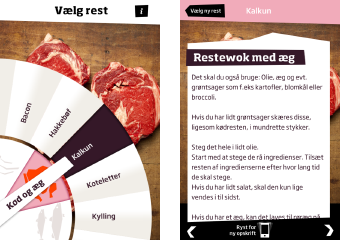
\includegraphics[scale=0.7]{billeder/forbilleder/forresten.png}
\capt{Brugergrænseflade i For Resten. Valg af rest (t.v.) og visning af opskrift (t.h.)}
\label{fig:forresten}
\end{figure}

For hver rest er der ca. 4 - 5 opskrifter, hvilket med 124 rester giver et samlet antal opskrifter på omkring 500 - 600 (dette er vores eget bud på mængden. Det faktiske antal opskrifter er ikke oplyst nogen steder). For opskrifterne vises der kun fremgangsmåde, og ikke en liste over ingredienser. Det er derfor heller ikke muligt at op- eller nedskalere opskrifsportionerne. Derudover er der ingen mulighed for at favorisere opskrifter eller på anden måde gemme resultater af en søgning. I forhold til søgningen så kan man, som sagt, kun søge på én enkelt rest, og ikke sammensætte rester, som ved andre løsninger. Samtidig har man kun mulighed for at vælge sin rest på hjulene, og har altså ikke muligheden for at skrive i et felt. Under afprøvningen var det derfor i nogle tilfælde svært at finde den ønskede ingrediens. Det er de samme problemstillinger, der kommer til udtryk i brugernes anmeldelser af app’en på Google Play. \Fx skriver brugeren \textit{TJA} \cite{tja}:

\begin{quote}
``Fin ide, men den burde være blevet kælet lidt mere for, før den røg i play. Hvem laver restemad af én rest og så en masse ting der skal købes? Jeg har brug for at kunne søge på tre-fire rester for at se, hvordan de kan kombineres til noget spændende. Og hvis jeg finder en opskrift, jeg vil prøve, så kan jeg ikke gemme den i appen, men skal søge den frem igen når jeg står i netto og skal købe de ting, der skal til - og søge den frem igen, når jeg skal lave maden. Alt for besværligt.''
\end{quote}

Sammenlagt har app’en på Google Play bedømmelsen 2,4 stjerner ud af 5, baseret på 69 bedømmelser, hvoraf næsten halvdelen kun har givet app’en 1 stjerne. Et andet kritikpunkt, der kommer til udtryk i flere anmeldelser, er, at app’en bruger for mange systemressourcer og er langsom til at starte op.

\subsection{DK-Kogebogen}
\label{subsec:dk-kogebogen}

DK-Kogebogen er en webapplikation, som tilbyder en lang række funktioner, hvoraf ``Tøm køleskabet'' er en af dem. Udover ``Tøm køleskabet'', tilbyder DK-kogebogen også en ugentlig madplan, en ekstern hjemmeside med fokus på viden omkring mad (energiindhold, vitaminindhold osv.), en kalorieberegner og meget meget mere. Sagt med andre ord, så prioriterer DK-Kogebogen ikke udelukkende sine ressourcer på ``Tøm køleskabet'', og dette kan påvirke kvaliteten af denne. Desuden kan det også være svært at skabe sig et overblik på hjemmesiden, da der er så mange funktioner pakket sammen på samme side. Siden har et omfang af 36.434 opskrifter, hvilket er det klart største antal blandt de undersøgte systemer. De mange opskrifter er indsendt og lavet af brugere af hjemmesiden. Dette kan både være positivt og negativt. Det kan være negativt, da der kan forekomme en del fejl i opskrifterne. DK-Kogebogen skriver på deres hjemmeside, om de indsendte opskrifter:

%kilde: http://www.dk-kogebogen.dk/opskrifts-service/indsend-opskrift.php
\begin{quote}
``Opskriften kan ses med det samme, men der vil senere blive rettet lidt til i teksterne.'' \cite{dk-kog-indtastopskrift}
\end{quote}

Det er altså muligt for alle at indsende opskrifter, som er fulde af fejl, og disse vil alligevel være synlige på siden. Til gengæld skaber det mulighed for, at den enkelte bruger føler sig mere knyttet til siden, da han/hun har et personligt engagement i den, fordi de indsender deres egne opskrifter; og dette vil resultere i en overordnet højere brugeraktivitet. Det skal noteres, at de 36.434 opskrifter ikke er unikke. Det vil sige, at der godt kan eksistere flere forskellige varianter af den samme opskrift; \fx er der 17 forskellige varianter af Boller i Karry, hvilket kan virke uoverskueligt.

Når brugeren vil anvende ``Tøm køleskabs''-funktionen, mødes vedkommende af følgende billede \ref{fig:dk-kogebogen1}, som er taget fra toppen af DK-Kogebogens forside. Her kan brugeren indtaste så mange ingredienser der er brug for, inden for en grænse på 55 karakter. For at systemet kan identificere ingredienser, skal der mellem hver ingrediens, som brugeren indtaster, være et mellemrumstegn. Begrænsningen på 55 karakter betyder, at der maksimalt kan søges på ca. 8-10 ingredienser af gangen (Forudsat at ingrediensnavne er 5-7 bogstaver lange).

\begin{figure}[H]
\centering

\includegraphics[scale=0.7]{billeder/forbilleder/dk-kogebogen.png}
\capt{DK-Kogebogens ``Tøm køleskabet''-funktion. Funktionen er tilgængelig i toppen af forsiden, og enhver anden underside.}
\label{fig:dk-kogebogen1}
\end{figure}

Efter brugeren har søgt på opskrifter med en eller flere specifikke ingredienser, viser DK-Kogebogen en liste med alle de opskrifter, som indeholder ingredienserne. På \figref{fig:dk-kogebogen2} ses en del af den liste, som er resultatet ved søgning på ``Tomat, Paprika og Kartoffel''. Ud fra opskrifterne kan der findes et kamera-symbol og/eller et dokument-symbol, som respektivt fortæller brugeren, om der er et billede af den pågældende opskrift, og/eller at opskriftens næringsindhold er beregnet og vist.


\begin{figure}[H]
\centering
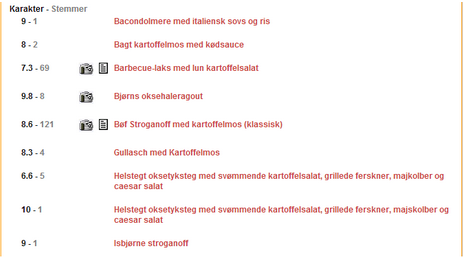
\includegraphics[scale=0.7]{billeder/forbilleder/dk-kogebogen2.png}
\capt{Liste af opskrifter, som indeholder ingredienserne Tomat, Paprika og Kartoffel.}
\label{fig:dk-kogebogen2}
\end{figure}

Brugeren vælger derefter en af opskrifterne han/hun finder mest interessant. Der er ikke overensstemmelse med, hvad \fx portionerne skal angives i. Inde på hjemmesiden er det i nogle tilfælde muligt at op- eller nedskalere portionsstørrelsen, mens der i andre tilfælde skaleres på antal personer. Derudover er der også nogle opskrifter, hvor det slet ikke er muligt at skalere. Her er brugeren i stedet for tvunget til selv at finde ud af, hvor stor en portion opskriften ca. passer til. Denne mangel på konsistens er endnu en af problematikkerne ved, at det er brugerne selv, som indsender opskrifterne. En endelig vurdering af DK-Kogebogen, vil kunne findes i \secref{subsec:eksisterende.sammendrag}.

\subsection{Opskrifter.dk}
\label{subsec:opskrifterdk}

Opskrifter.dk er endnu en webapplikation, der tilbyder en ``Tøm køleskabet''-funktion, som kan bruges til at finde opskrifter i deres samling af opskrifter. Ligesom i For Resten kan ingredienser kun vælges fra kategorier, dog er der i dette system hele 624 ingredienser, fordelt over 27 kategorier. Modsat For Resten kan man her vælge mere end én ingrediens. Dette gøres ved først at vælge en kategori og derefter finde og vælge en ingrediens og klikke på knappen ``Tilføj >''. Man kan ligeledes fjerne allerede valgte ingredienser ved at markere dem og klikke på knappen ``< Fjern'', eller fjerne alle valgte ingredienser ved at klikke på knappen ``< Fjern alle''. Når man har valgt de ingredienser, man ønsker at inkludere, kan man foretage sin søgning ved at klike på knappen ``Søg''. 

\begin{figure}[H]
\centering
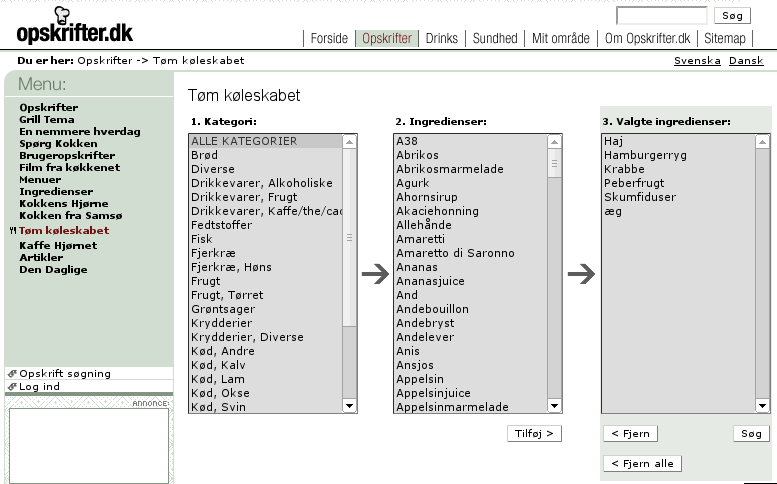
\includegraphics[scale=0.6]{billeder/forbilleder/opskrifterdk.png}
\capt{Brugergrænsefladen for Opskrifter.dk’s ``Tøm køleskabet''-funktion.}
\label{fig:opskrifterdk1}
\end{figure}

Søgningen foretages blandt de ca. 2700 opskrifter, som er tilgængelige på Opskrifter.dk. Resultaterne vælges ud fra, om de inkluderer minimum én af de valgte ingredienser. Under hver opskriftnavn vises antallet af valgte ingredienser, som opskriften inkluderer, men det er umiddelbart ikke muligt at sortere resultaterne efter dette tal. Klikker man på et resultat, åbnes den valgte opskrift til højre for resultaterne, og altså ikke på en ny side eller i et nyt vindue/faneblad. Opskrifterne viser informationer såsom tilberedningstid samt alle ingredienserne og deres mængder. Det er på alle opskrifter muligt at skalere opskriften til et bestemt antal personer. Figur \ref{fig:opskrifterdk2} viser et eksempel af et søgningsresultat. 

Kvaliteten af opskrifterne er forholdsvis høj og ca. 40 \% af alle opskrifter er med billede. Dette skyldes sandsynligvis, at det ikke er muligt for almindelige brugere direkte at indsende opskrifter. Almindelige brugere kan derimod indsende opskriftforslag, som først skal gennemlæses og tilføjes af en administrator.

\begin{figure}
\centering
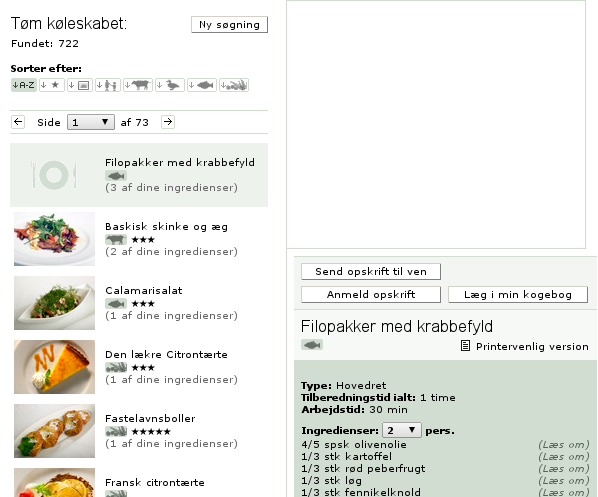
\includegraphics[scale=0.7]{billeder/forbilleder/opskrifterdk2.png}
\capt{Resultatsiden vist ved søgning med Opskrifter.dk’s ``Tøm køleskabet''-funktion. Her er markeret en opskrift, der ikke indeholder et billede af retten.}
\label{fig:opskrifterdk2}
\end{figure}

Opskrifter.dk har også et brugersystem, der tillader brugere at registrere sig og logge ind. Dette giver mulighed for, at man bl.a. kan gemme de opskrifter, man har fundet (ved at klikke på ``Læg i min kogebog''). Derudover husker ``Tøm køleskabet''-funktionen de ingredienser, man har indtastet, til næste gang man besøger siden.
Under ``Tøm køleskabet''-funktionen er det også muligt for brugeren at skrive kommentarer til funktionen. Disse kommentarer har givet et indblik i, hvad Opskrifter.dk’s brugere synes om funktionaliteten. Nogle kommentarer går på manglende ingredienser, mens en stor del kommentarer går på, at funktionen finder opskrifter, som man ikke kan lave uden at skulle købe en masse ind. \Fx skriver brugeren Jytte Hasselriis:

%kilde: http://opskrifter.dk/Toem-koeleskabet.149.0.html
\begin{quote}
``Hvordan skulle jeg kunne lave fasan i flødesovs, når jeg ikke har en fasan i køleskabet????'' \cite{opskrift-fasan}
\end{quote}

Dette synes at udtrykke en vis utilfredshed med den måde, hvorpå Opskrifter.dk’s ``Tøm køleskabet''-funktion vælger resultater på.
\subsection{Sammendrag}
\label{subsec:eksisterende.sammendrag}

De tre systemer; For Resten, DK-Kogebogen og Opskrifter.dk er i foregående afsnit blevet undersøgt og analyseret. Der er blevet lagt vægt på fire hovedpunkter: antallet af opskrifter i systemet, Kvaliteten af opskrifterne, systemets fleksibilitet og opskriftssøgningsfunktionen (også kaldet ``Tøm køleskabet''-funktionen). De fire hovedpunkter er specificeret i detaljer i \secref{sec:eksisterendesystemer}. For at skabe et samlet overblik, har vi valgt at samle de vigtigste og mest karakteristiske dele fra hver af systemerne i \tableref{table:sammentabel}.

\ourtable{sammentabel}{3}{Oversigt over opfyldelse af kriterier af de eksisterende systemer.}
                                            {System}
       { Funktioner                }{ For Resten   & DK-kogebogen   & Opskrifter.dk }{
\ourrow{ Kvalitet af opskrifter    }{ ringe        & svingende      & god           }
\ourrow{ Antal opskrifter          }{ 550          & 36.500         & 2.700         }
\ourrow{ Fleksibilitet             }{ meget ringe  & middel         & god           }
\ourrow{ Opskriftssøgningsfunktion }{ meget ringe  & middel         & middel        }
}

\begin{description}
\item[Kvalitet af opskrifter] \hfill \\
Kvaliteten af opskrifterne på DK-Kogebogen er meget varierende. Brugeren risikerer at støde på opskrifter, der slet ikke er brugelige. 

Kvaliteten af opskrifterne på For Resten kunne være meget bedre. Opskrifterne er udelukkende lavet eller tilføjet af folkene bag app’en, og derfor er opskrifternes opbygning og design konsistent, hvilket naturligvis havde været en god egenskab, hvis det ikke var for det faktum, at opbygningen er uoverskuelig, og at der ingen billeder eksisterer af opskriften. Der er ingen ingrediensliste på opskriften og beskrivelsen af fremgangsmåden er kortfattet. 

Kvaliteten af opskrifterne på Opskrifter.dk er høj. Dette skyldes, at opskrifterne bliver gennemgået af en administrator, inden de bliver tilgængelige på Opskrifter.dk’s side, hvilket er modsat af DK-Kogebogen, hvor opskrifterne bliver tilgængelige med det samme. Desuden er Opskrifter.dk’s opskriftsopbygning konsekvent i alle opskrifter, hvilket også er i modsætning til DK-Kogebogens opskrifter. Der mangler dog billeder på nogle opskrifter.

\item[Antal opskrifter] \hfill \\
Som det ses i \tableref{table:sammentabel}, har DK-Kogebogen det langt største antal opskrifter, mens Opskrifter.dk har ca. fem gange flere opskrifter end For Resten. Dermed har DK-Kogebogens ``Tøm køleskabet''-funktion også langt bedre chance for at give brugeren et resultat, når der søges på opskrifter med specifikke ingredienser.

\item[Fleksibilitet] \hfill \\
Der er stor forskel på fleksibiliteten fra system til system. I For Restens app, er det slet ikke muligt at skalere portionsstørrelse. På DK-Kogebogens side er det kun muligt med nogle opskrifter, mens det på Opskrifter.dk er muligt at skalere portionsstørrelse i alle opskrifter. Denne relativ simpel funktion ses som meget brugbar, da brugeren undgår selv at skulle gange ingrediensmængder op.

Kun Opskrifter.dk tilbyder brugeren muligheden for at sortere i resultaterne af en opskriftssøgning. Her kan der sorteres efter alfabetisk orden, opskrifter med billeder, opskrifter med kød samt flere. Som en bruger på Opskrifter.dk dog pointere, mangler den sorteringsmulighed, som sortere efter de opskrifter som indeholder flest af de ingredienser som brugeren har indtastet. Denne sorteringsmulighed anses for os, som værende den mest relevante, da man som bruger er interesseret i at få anvendt så mange af ens madrester som muligt.

\item[Opskriftssøgningsfunktion] \hfill \\
De tre systemer er vidt forskellige i deres måde at håndtere søgning på. Der er mellem DK-kogebogen og Opskrifter.dk en markant forskel på, hvordan resultater findes. I DK-Kogebogen findes kun opskrifter, som inkluderer alle de indtastede ingredienser, mens Opskrifter.dk finder alle opskrifter, som indeholder bare én af de valgte ingredienser. Dvs., at man med DK-Kogebogen får færre resultater jo flere ingredienser man skriver, mens det med Opskrifter.dk er direkte modsat, idet antallet af resultater stiger voldsomt med antallet af ingredienser, man skriver. Opskrifter.dk’s måde at gøre det på, kombineret med deres manglende sortering, giver en uoverskuelig mængde af resultater, hvor en stor del af disse måske kun indeholder en af de valgte ingredienser.
\end{description}

%Ud fra vores observationer af løsningernes fordele og ulemper, kan vi uddrage hvilke egenskaber vi ønsker at benytte i vores eget projekt. \Fx viser den generelle utilfredshed med Forbrugerstyrelsens mobilapp For Resten, at det er vigtigt med mange opskrifter og muligheden for at vælge mere end én rest. Observationerne af For Resten og Opskrifter.dk viser også, at brugergrænseflade er et vigtigt element. I disse to løsninger skal man vælge ingredienser ved at lede rundt i kategorier. Dette føles meget ineffektivt i forhold til at skrive navnet på ingrediensen på et tastatur.

%Af dette kan man aflede, at en kombination af de to må være den optimale løsning. Har man valgt få ingredienser, er man sandsynligvis interesseret i at få vist resultater som indeholder alle de ingredienser man har valgt. Har man derimod valgt mange ingredienser, er man interesseret i at få vist resultater som indeholder flest muligt af de ingredienser man har valgt.

%Som det ses i \tableref{table:sammentabel}, har DK-Kogebogen det langt største antal opskrifter, mens Opskrifter.dk har ca. fem gange flere opskrifter end For Resten. Dermed har DK-Kogebogens ``Tøm køleskabet''-funktion også langt bedre chance for at give brugeren et resultat, når han/hun søger på opskrifter med specifikke ingredienser. Til gengæld er kvaliteten af opskrifterne på DK-Kogebogen meget varierende, og derfor kan brugeren risikere at støde på opskrifter, som er dårlige eller ubrugelige. Kvaliteten af opskrifterne på For Resten er sammenlagt dårlig. Opskrifterne er udelukkende lavet eller tilføjet af folkene bag app’en, og derfor er opskrifternes opbygning og design konsistent, hvilket naturligvis havde været en god egenskab, hvis det ikke var for det faktum, at opbygningen er uoverskuelig. Der er ingen ingrediensliste på opskriften og beskrivelsen af fremgangsmåden er kortfattet. Kvaliteten af opskrifterne på Opskrifter.dk er høj. Dette skyldes, at opskrifterne bliver gennemgået af en administrator, inden de bliver tilgængelige på Opskrifter.dk’s side, hvilket er modsat af DK-Kogebogen, hvor opskrifterne bliver tilgængelige med det samme. Desuden er Opskrifter.dk’s opskriftopbygning konsekvent i alle opskrifter, hvilket også er i modsætning til DK-Kogebogens opskrifter.

%Der er stor forskel på fleksibiliteten fra system til system. I For Restens app, er det slet ikke muligt at skalere portionsstørrelse. På DK-Kogebogens side er det kun muligt med nogle opskrifter, mens det på Opskrifter.dk er muligt at skalere portionsstørrelse alle opskrifter. Det er en funktion, som er meget brugbar, da man som bruger ikke ønsker at bruge en masse tid på selv at beregne en passende portionsstørrelse. Af sorteringsmuligheder af opskriftresultaterne, er det kun Opskrifter.dk som tilbyder denne mulighed. Her kan der sorteres efter alfabetisk orden, opskrifter med billeder, opskrifter med kød samt flere. Som en bruger på Opskrifter.dk dog pointere, mangler den sorteringsmulighed, som sortere efter de opskrifter som indeholder flest af de ingredienser som brugeren har indtastet. Denne sorteringsmulighed anses for os, som værende den mest relevante, da man som bruger er interesseret i at få anvendt så mange af ens madrester som muligt. 

%De tre løsninger er vidt forskellige i deres måde at håndtere søgning på. Ud fra vores afprøvninger og observationer af løsningernes fordele og ulemper, kan vi uddrage hvilke egenskaber vi ønsker at benytte i vores eget projekt. \Fx viser den generelle utilfredshed med Forbrugerstyrelsens mobilapp For Resten, at det er vigtigt med mange opskrifter og muligheden for at vælge mere end en rest. Observationerne af For Resten og Opskrifter.dk viser også at brugergrænseflade er et vigtigt element. I disse to løsninger skal man vælge ingredienser ved at lede rundt i kategorier og i For Resten endda bevæge fingeren rundt i en cirkel for at rotere hjulene for kategorier og rester. Dette føles meget ineffektivt i forhold til at skrive navnet på ingrediensen på et tastatur. Derudover er der mellem DK-kogebogen og Opskrifter.dk en markant forskel på hvordan resultater findes. I DK-kogebogen findes kun opskrifter som inkluderer alle de indtastede ingredienser, mens Opskrifter.dk finder alle opskrifter som indeholder bare én af de valgte ingredienser. Dvs. at man med DK-kogebogen får færre resultater jo flere ingredienser man skriver, mens det med Opskrifter.dk er direkte modsat, idet antallet af resultater stiger voldsomt med antallet af ingredienser man skriver. Opskrifter.dk’s måde at gøre det på, kombineret med deres manglende sortering, giver et stor uoverskuelig mængde af resultater, hvor en stor del af disse måske kun indeholder en af de valgte ingredienser. Af dette kan man aflede at en kombination af de to må være den optimale løsning. Har man valgt få ingredienser, er man sandsynligvis interesseret i at få vist resultater som indeholder alle de ingredienser man har valgt. Har man derimod valgt mange ingredienser, er man interesseret i at få vist resultater som indeholder flest muligt af de ingredienser man har valgt.


\section{Systemdefinition}

%Systemdefinitionen nedenunder er en naturlig og kortfattet beskrivelse af den løsning, vi ønsker at fremstille. Den er baseret på gruppens egne ønsker om projektretning og interviews med gruppens to informanter. BATOFF-modellen er blevet brugt til at formulere systemdefinitionen. BATOFF indeholdholder følgende punkter: \emph{\textbf{b}etingelser}, \emph{\textbf{a}nvendelsesområde}, \emph{\textbf{t}eknologier}, \emph{\textbf{f}unktioner}, \emph{\textbf{f}ilosofi}. Gruppen benytter BATOFF-modellen fordi det fastsætter nogle rammer i forhold til opsætningen og indholdet af systemdefinitionen samt opretter en form for standard, der gør det muligt at sammenligne flere forskellige systemdefinitioner på en logisk måde.

%Efter møde 1 (se bilag) med vores informanter, har gruppen fået forståelse for at madspild er et reelt problem for dem. Det er blevet forklaret hvad der ofte er grunden til madspildet, og på baggrund af møde 1 er to systemdefinitioner blevet konstrueret. Blandt de to systemdefinitioner valgte informanterne systemdefinition 1. Systemdefinition 2 kan ses i den akademiske rapport.

%Systemdefinition er defineret som følgende:

%\begin{quote}
%Systemet skal fungere som et online opskriftsregister, der giver brugeren idéer til opskrifter han rent faktisk kan lave ud fra de madvarer han har. Systemet fokuserer på at mindske madspild, da forbrugere smider mad ud på grund af et manglende formål med anvendelsen af resterne. Brugerne af programmet er en del af en husholdning og vil have meget varierende erfaringer inden for brug af internettet. Udviklerne af systemet er ulønnede studerende. Deadline for det færdige system kan ikke ændres. Systemet skal køre på en server, der kan tilgås via en webapplikation fra en internetbrowser på enhver type computer. På baggrund af en mængde fødevarer som input, findes forskellige opskrifter, der bedst muligt matcher disse. Opskrifterne skal kunne sorteres på flere måder, og ingredienser skal kunne huskes til næste gang, hvis ønsket.
%\end{quote}

%Gruppen mødtes anden gang med informanterne efter at have fremstillet de to systemdefinitioner for at få feedback på projektets retning og få valgt et attraktivt systemdefinition. Formålet med mødet er at fortælle informanterne om gruppens idé om en opskriftssøgemaskine, der kun finder opskrifter man kan lave ud fra de råvarer, man har til rådighed. Gruppen vil høre om informanterne ville kunne bruge et sådan system. Gruppen holder sig på nuværende tidspunkt meget åbent, da gruppen vil gerne gøre det muligt for informanterne at komme med nye idéer, også selvom de er markant anderledes fra gruppens initierende problemstilling og systemdefinitioner. Derfor foregår mødet som et semistruktureret interview. Det er vigtigt for gruppen at få informanternes idéer til hvilke funktioner et sådan system skal have og hvilken krav, de stiller.

%Møde 2 gjorde det klart, at informanterne ser systemdefinition 1 som et meget brugbart system. Vi er blevet præsenteret for en masse funktioner, som hver informant har ønsket til et sådan system.

%Dokumentation og referater fra møde 1 og 2 samt alle efterfølgende møder med informanterne kan findes i \apref{ap:informant}.

\section{Prototyper}
\label{sec:prototyper}

Vi udarbejdede to prototyper, der fokuserede på søgefunktionaliteten, som bliver præsenteret i \secref{subsec:prototype1}, og en større prototype, der fokuserede på systemets andre funktioner, som bliver præsenteret i \secref{subsec:prototype2}.

Vi udførte prototypeafprøvningerne hjemme hos begge informanter (en af gangen). 
Informanterne blev bedt om at udføre en case, som havde til formål at få dem igennem prototyperne, så vi havde mulighed for at overvåge dem, og efterfølgende diskutere prototyperne med dem.
Afprøvningerne er dokumenteret ved hjælp af videooptagelser, som refereres til i \apref{ap:prototype1} for prototyperne, der havde fokus på søgefunktionalitet, og i \apref{ap:prototype2} for prototypen, der havde fokus på systemets andre funktioner.

Prototyperne med fokus på søgefunktionalitet blev afprøvet i første fase af projektforløbet, og prototypen med fokus på systemets andre funktioner blev afprøvet i anden fase, hvilket også er illustreret i \tableref{table:iterationeroverblik} i \secref{sec:evolution}.


\section{Prototype 1}
\label{ap:prototype1}

Afprøvning af Prorotype 1A på Merete er blevet filmet. Klippet kan ses på Youtube: \url{http://youtube.com/watch?v=E-8WA6QrZo4}

Afprøvning af Prorotype 1B på Merete er blevet filmet. Klippet kan ses på Youtube: \url{http://youtube.com/watch?v=rUJexwTpu48}

\begin{description}
\item[Formål] Vores system kan ikke benyttes uden at brugeren indtaster en mængde ingredienser, som de vil udføre en søgning på. For at tilbyde en brugervenlig metode til indtastning af disse ingredienser vil vi gerne teste 2 forskellige metoder på informanterne. Disse 2 metoder testes med hver deres prototype i papirsform, prototype 1A og 1B.
\item[Prototype 1A]

\begin{figure}[H]
\centering
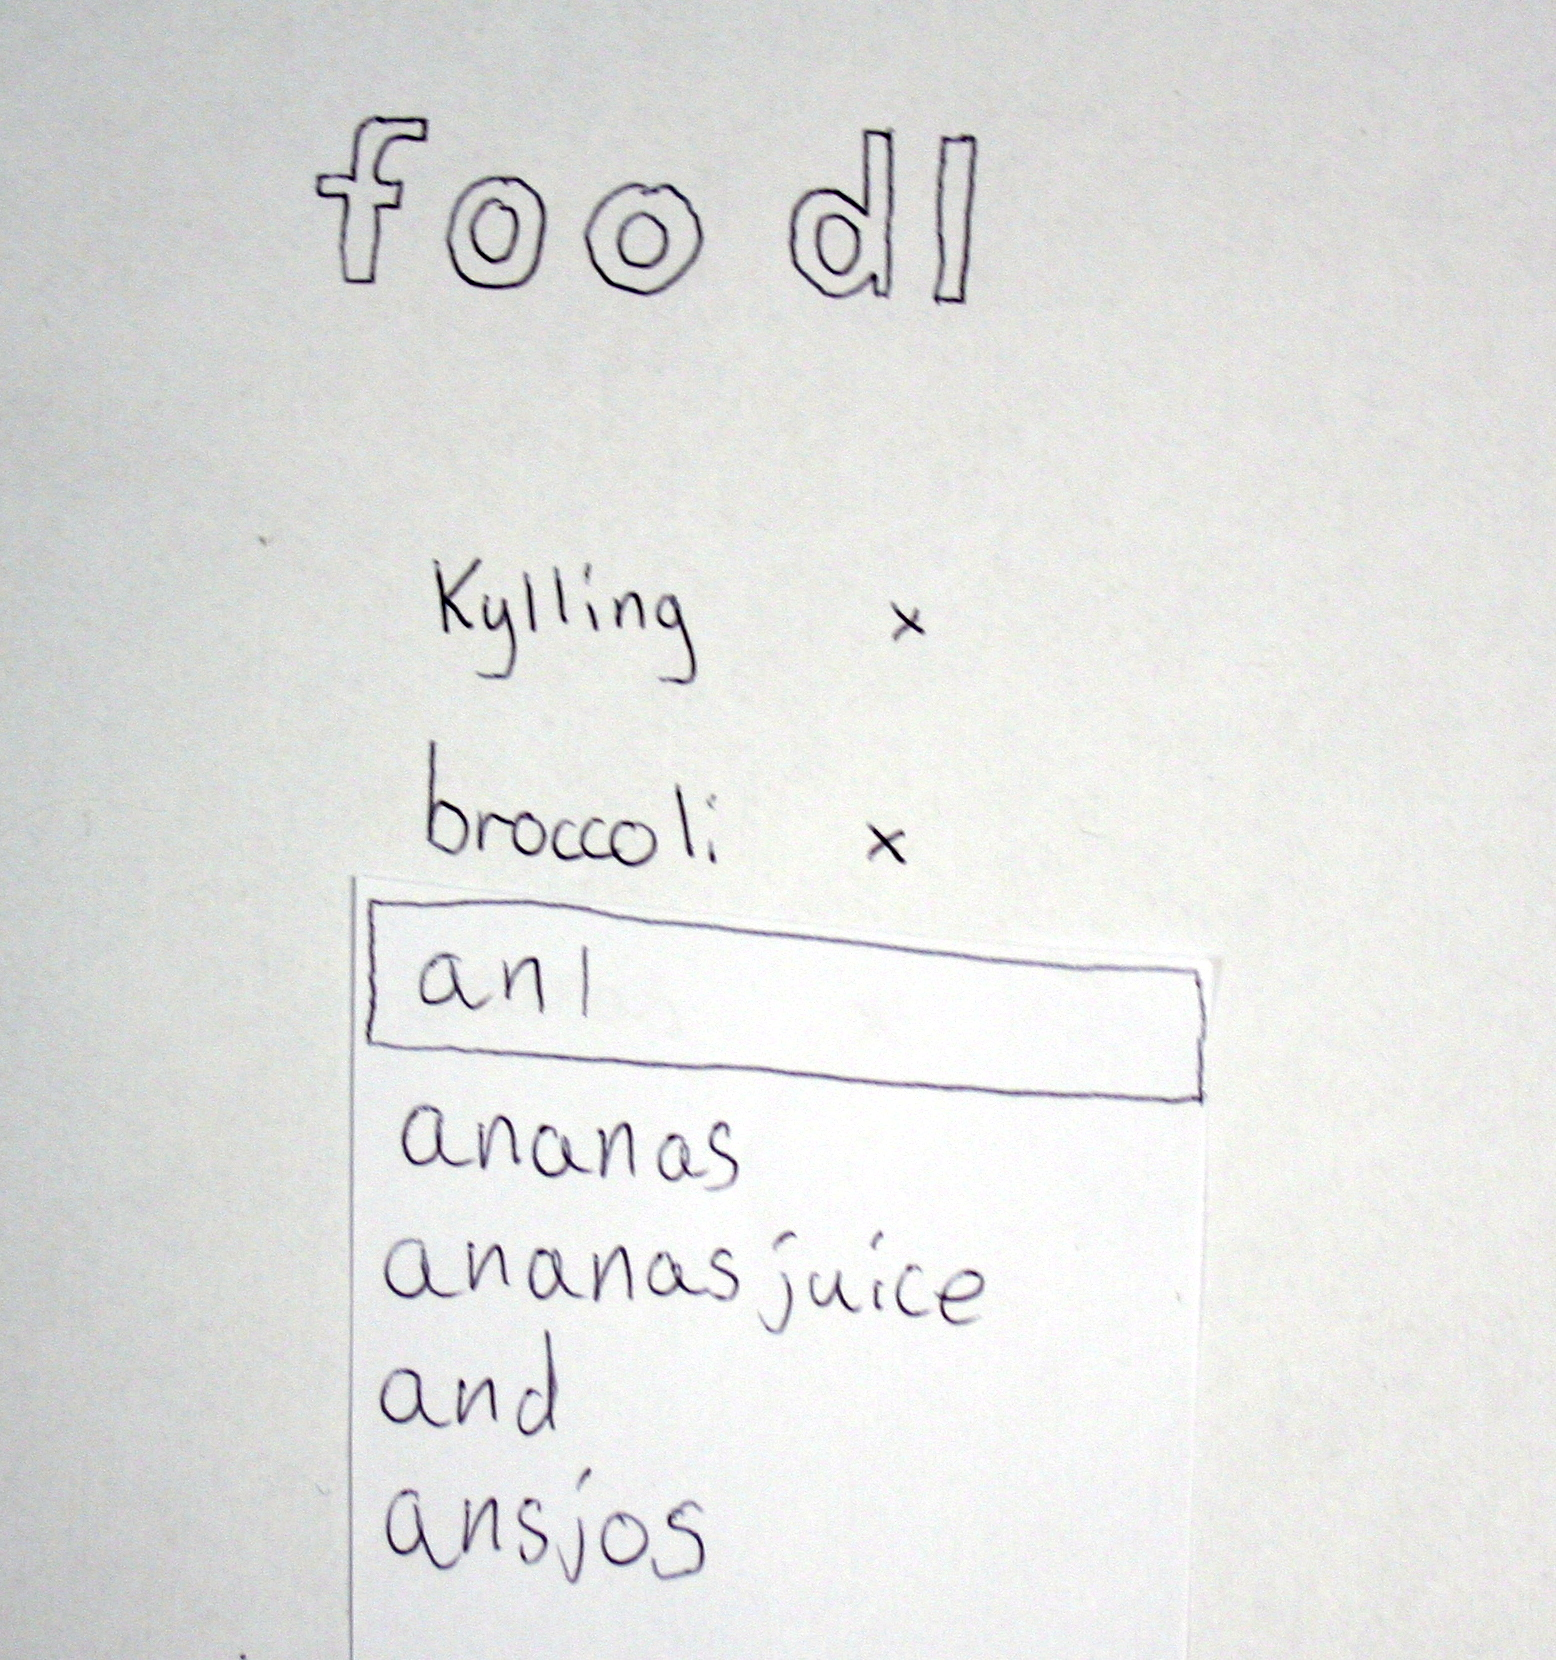
\includegraphics[width=0.5\textwidth]{billeder/prototyper/prototype1a.jpg}
\capt{Visualisering af prototype 1A.}
\label{fig:prototype1a}
\end{figure}

Præsenterer en søgeboks for brugeren, der minder meget om Google’s søgefelt. Når man indtaster et bogstav, fx “k”, kommer der en række forslag frem, såsom kylling og kartoffel, også på samme måde som ved Google, blot med den forskel at der kun foreslås ingredienser. Man kan nu klikke på forslaget eller trykke enter. Man kan også skrive ingrediensens navn færdig manuelt.

Tanken bag denne metode er at man hurtigt kan indtaste en ingrediens hvis man blot ved hvordan de første få bogstaver staves. Brugeren har med stor sandsynlighed kendskab til denne metode, da den bruges af Google, og samtidig har vi også konstrueret logoet og sidens design så det også minder om Google, netop for at gøre det intuitivt for brugeren.

Ulempen er at man har brug for et tastatur og skal tænke over hvordan man staver til ingrediensen. Det er også muligt at overse forslagene og tro man er nødsaget til at stave et meget langt ord, som for eksempel 

\item[Prototype 1B]

\begin{figure}[H]
\centering
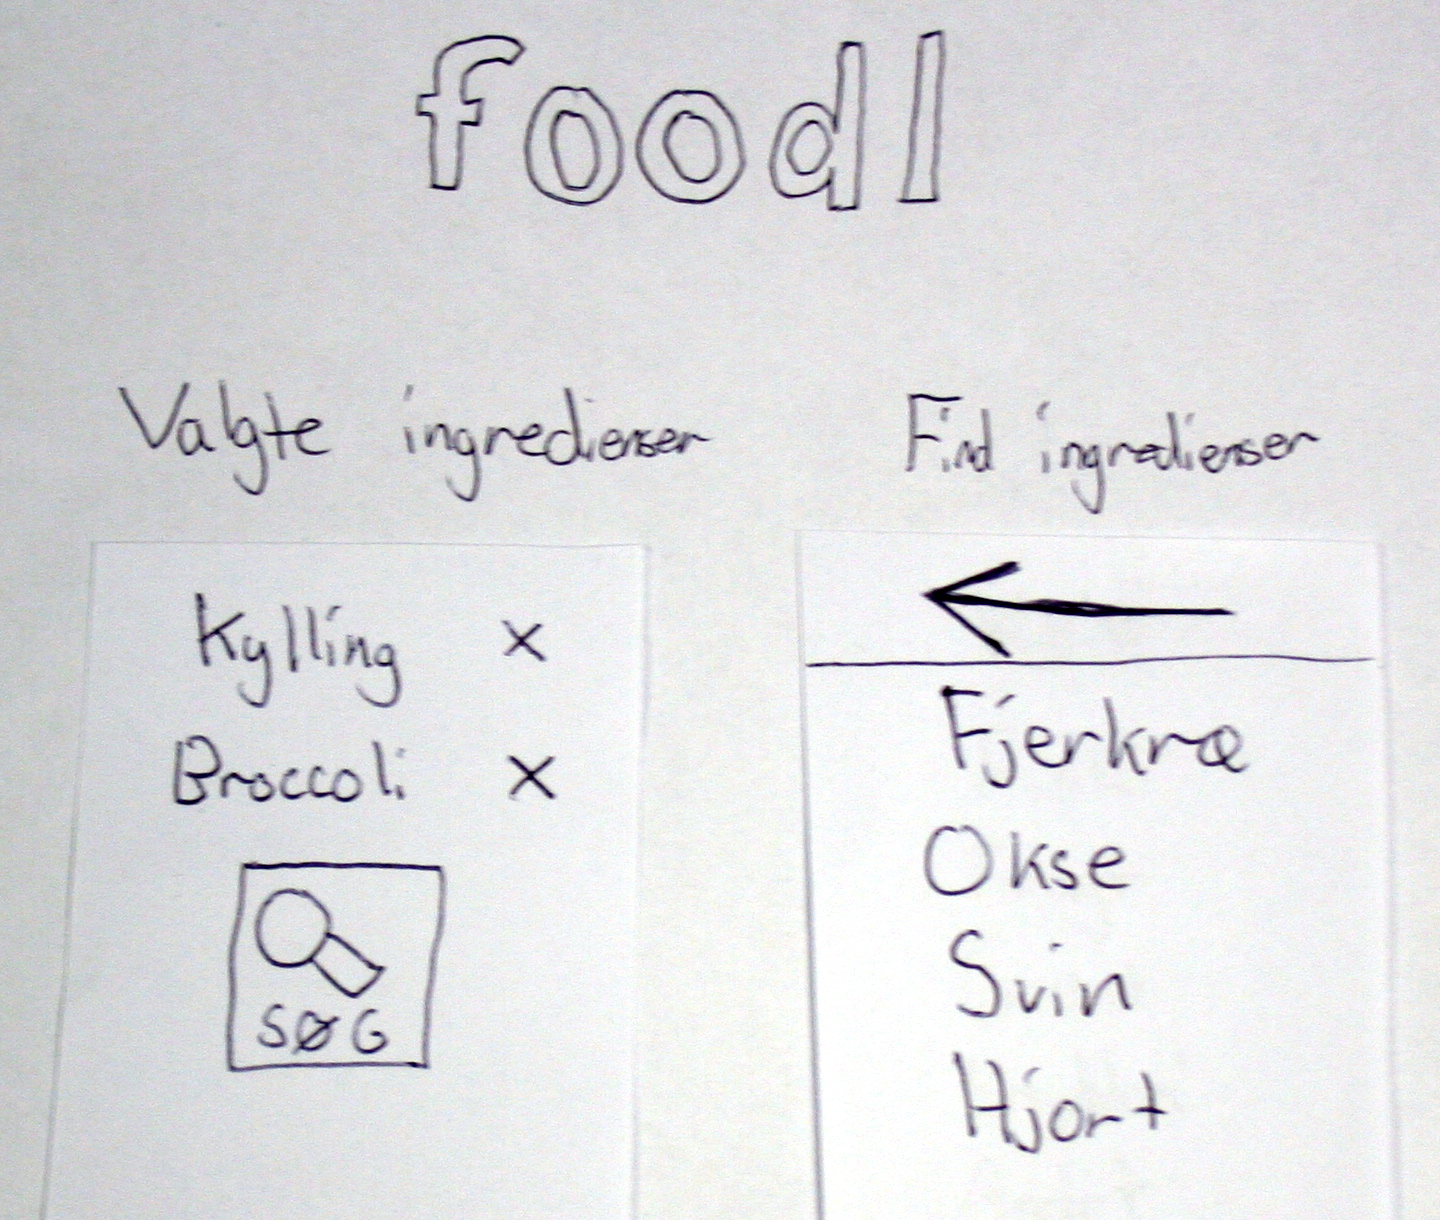
\includegraphics[width=0.5\textwidth]{billeder/prototyper/prototype1b.jpg}
\capt{Visualisering af prototype 1B.}
\label{fig:prototype1b}
\end{figure}

Fokuserer på et valg af ingredienser blandt kategorier. Man vælger først en bred kategori, som for eksempel fjerkræ, kød, brød, frugt og grønt. Dernæst vælger man et antal gange en underkategori, indtil man til sidst kan vælge en ingrediens fra en liste.

Fordelen ved denne metode er at brugeren ikke har behov for et tastatur. Det er også nemt at benytte på tablets og smartphones, da der kan skal klikkes. Ulempen er muligheden for mange kategori og forvirring omkring hvilken kategori en ingrediens findes i. Måske vil den sidste kategori der vælges stadig indeholde rigtig mange ignredienser, sådan at man skal bladre i denne liste for at finde den ønskede ingrediens. 

\item[Sammendrag] Prototype 1A var hurtig, nem og effektiv. Informanten kunne bedst lide denne metode, og hun havde ikke brug for vejledning for at kunne finde de 3 ingredienser kylling, ananas og broccoli.

Prototype 1B var langsommere at bruge og informanten syntes ikke om den. Hun var i tvivl om hvilken kategori hun skulle vælge kylling under. Kategorierne kan laves på mange forskellige måder, og uanset hvordan de vælges, vil der med garanti være nogle brugere der er i tvivl om hvor de skal lede efter en bestemt ingrediens. Et eksempel kan være kartoffelstivelse. Nogle vil lede efter kartoffelstivelse i kategorien grøntsager (fordi kartofler findes der), mens andre måske vil lede efter en kategori med navnet brød og gryn.

På baggrund af informantens valg, vælger vi at benytte metoden fra prototype 1A til at vælge ingredienser.
\end{description}

\section{Prototype 2}

Afprøvning af prototype 2 m/ fokus på systemets funktioner

\begin{description}
\item[Formål] På baggrund af møde 2, hvor informanterne kom med krav til systemets funktioner, har vi nu lavet en diasshow-prototype på gomockingbird.com, hvor systemets funktion er vist. Når informanterne præsenteres for funktionerne i noget der, med lidt god vilje, ligner et rigtigt program, så kan det være at informanten bliver klar over at en funktion enten mangler, eller at en tidligere foreslået funktion er overflødig. Formålet med mødet er derfor primært at ud af, om der er de funktioner, som informanten har brug for. Derudover vil vi også gerne finde ud af om brugeren kan finde de nødvendige funktioner, altså om programmet og dets funktioner som helhed er intuitive at bruge for informanterne.

\begin{figure}[H]
\centering
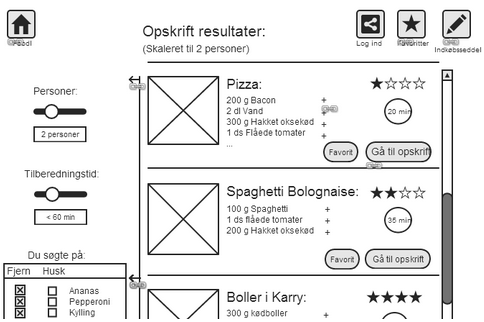
\includegraphics[scale=0.7]{billeder/prototyper/prototype2.png}
\capt{Visualisering af prototype 2.}
\label{fig:prototype2}
\end{figure}

Først udføres en case for at få ledt brugeren rundt blandt alle funktionerne.

\item[Case] Følgende case blev udført af informanterne.

\begin{enumerate}[noitemsep]
\item Udfør en søgning på ingredienserne (pepperoni, ananas og kylling). Ingredienser tilføjes ved at klikke i søgefeltet
\item Skjul alle opskrifter med nødder
\item Gå til den første opskrift, der fremkommer
\item Gå tilbage og tilføj 200 g Bacon (fra pizzaens ingredienser) til din indkøbsliste
\item Print indkøbslisten ud
\item Gør klar til en helt ny søgning
\item Foretag en søgning på pepperoni
\item Du fandt ingen opskrifter, så du vil gerne tilføj ananas, inden du søger igen (du søger altså på pepperoni og ananas)
\item Føj den første opskrift, du finder, til dine favoritter
\end{enumerate}

Efter casen tages en snak om hver af disse funktioner og muligheder med systemet.

Informanten bliver præsenteret for mange funktioner, hvor vi her beskriver hvad deres mening var omkring disse funktioner efter at have udført casen.

\begin{itemize}[noitemsep]
\item Begrænse søgeresultat efter tilberedningstid
\begin{itemize}[noitemsep]
\item Merete synes idéen er god, men foreslår nu kun 2 valgmuligheder ``kort'' eller ``lang'' tilberedningstid
\item Keld synes også dette er en god ide. En opdeling på en 30 min. burde være fint, måske 15 min. Hvis det er tilberedningstid på over en time, må skalaen godt springe mere end 15-30 min.
\end{itemize}
\item Sidebar
\begin{itemize}[noitemsep]
\item Merete opdagede ikke at denne sidebar kunne trækkes ud
\item Den ligger ikke logisk for en. Selvom den er stor. Den bliver skjult i designet
\item Keld synes ikke det ser for rodet ud, selvom sidebaren er ude hele tiden
\end{itemize}
\item Skalere en opskrift til x personer
\begin{itemize}[noitemsep]
\item Merete ser det som en nyttig funktion, hun vil skalere til mellem 2-4 personer
\item Det er en god funktion, som Keld er sikker på mange vil få brug for. Opskalering til 5 burde være nok. Måske 1-20, så er gæstebehov også dækket ind. Men det er trods alt til rester, så til 5 personer burde være nok.
\end{itemize}
\item Fjerne ingredienser inden en søgning udføres (på forsiden)
\begin{itemize}[noitemsep]
\item Merete synes det er meget brugbart
\item Keld synes det er fint at det er på forsiden
\end{itemize}
\item Fjerne ingredienser efter en søgning er udført (på søgeresultatsiden)
\begin{itemize}[noitemsep]
\item Merete synes idéen med at kunne fjerne ingredienser mens der vises søgeresultater er god
\item Keld synes det er fint, at det også er muligt i sidebaren
\end{itemize}
\item Huske ingredienser til næste søgning
\begin{itemize}[noitemsep]
\item Merete synes måden det fungerer på i prototypen er god. Hun vil ikke have at de huskede ingredienser vises på forsiden
\item Keld synes det er rart at det er muligt at huske nogle ingredienser. Det ville måske også være rart, hvis det også var muligt at gøre fra forsiden. Keld er dog i tvivl om, hvor på forsiden det skulle være. Det er måske alligevel bedst hvis forsiden er simpel. Han synes funktionen er brugbar
\end{itemize}
\item Skjule opskrifter indeholdende bestemte ting
\begin{itemize}[noitemsep]
\item Merete synes det virker godt
\item Keld synes det er en god ide. Han fik hurtigt fundet funktionen, så snart toolboxen blev åbnet
\end{itemize}
\item Browsers tilbageknap går til forsiden (beholder ingredienser)
\begin{itemize}[noitemsep]
\item Merete opdagede ikke denne funktion
\item Keld opdagede funktionen, og anvendte den også. Måske ville en tilbage- og fremknap på selve siden være brugbar, foreslår Keld
\end{itemize}
\item Home knap går tilbage (fjerne ingredienser)
\begin{itemize}[noitemsep]
\item Merete synes det virkede naturligt
\item Keld synes det er godt at have en kanp som går helt tilbage. Men han foreslår endnu engang at have en frem- og tilbageknap som supplerer home-knappen
\end{itemize}
\item Visning af opskrifter (ekspander ved mouse over)
\begin{itemize}[noitemsep]
\item Merete synes opskrifterne blev vist fint. Hun kunne godt lide idéen med at ekspandere opskriften ved mouseover
\item Keld synes bare man skal have vist de væsentligste ingredienser. Han synes det ville være smart, hvis det var muligt at se hele ingredienslisten ved hjælp af et mouse-over
\end{itemize}
\item Gå til opskrifter (evt link ved klik på navn)
\begin{itemize}[noitemsep]
\item Merete synes ikke knappen “Gå til opskrift”, er overflødig. Hun ville blive forvirret hvis den ikke var der, og man bare skulle trykke et sted på opskriften (navnet, eller baggrunden, hvor baggrundsfarve ændrer sig eller lignende)
\item Keld synes det er godt med en “Gå til opskrift”-knap. Det er brugervenligt
\end{itemize}
\item Tilføj opskrift til favoritter
\begin{itemize}[noitemsep]
\item Merete synes ikke man skal gå fra et søgeresultat og over til favoritsiden hver gang man tilføjer en opskrift til favoritter. Opskriften skal blot tilføjes. Måske den skal sige en lyd og fjerne knappen man trykkede på. Favoritter-ikonet kunne lyse op
\item Skal lave en “Fjern fra favorit-knap”, så man hurtigt kan ombestemme sig
\item Keld synes det er smart nok at man sendes ind på favoritlisten, så man er sikker på at opskriften er kommet derind. Havde man samtidig en frem- og tilbageknap ville det være endnu bedre
\end{itemize}
\item Favoritter (knappen, der viser ens favoritter)
\begin{itemize}[noitemsep]
\item Merete var lidt forvirret med hensyn til om den tilføjede en opskrift til favoritter, eller hvad den gjorde
\item Keld synes at det skal være muligt at skalere opskrifterne på favoritsiden og at det er muligt nemt at fjerne opskrift fra favoritsiden igen
\end{itemize}
\item Visning af favoritter (layout)
\begin{itemize}[noitemsep]
\item Merete syntes layoutet var godt, og kunne godt lide at det mindede om layoutet ved visning af søgeresultat
\item Keld synes godt om layoutet
\end{itemize}
\item Visning af indkøbsliste
\begin{itemize}[noitemsep]
\item Merete synes det er en god idé at man kan tilføje tekst
\item Keld foreslår at man har ingredienslisten fra den opskrift man har været inde på, ved siden af indkøbslisten, så det er muligt hurtigt at tilføje flere ingredienser derfra
\item Keld synes indkøbslisten er meget brugbar. Det er for ofte man glemmer nogle ting, uden indkøbslisten
\end{itemize}
\item Tilføje opskrifts ingredienser til indkøbsliste
\begin{itemize}[noitemsep]
\item Merete vidste ikke hvordan man gjorde. Hun troede ikke man kunne trykke på +’et
\item Keld kunne godt tilføje en ingrediens til indkøbslisten
\end{itemize}
\item Home-knappen sender en til en helt tom forside
\begin{itemize}[noitemsep]
\item Merete kunne godt lide dette. Det virkede helt naturligt for hende
\item Keld synes det giver mening
\end{itemize}
\item Logge ind (få afklaret med brugeren, hvordan det skal foregå)
\begin{itemize}[noitemsep]
\item Log ind mest forståeligt
\item Kender meget til login, intet til synkronisering
\item Log ind er klart mest forståeligt for Keld. Keld har ikke lyst til at indtaste mere end mail-adresse, navn eller brugernavn og adgangskode. Helst ikke mere end det. Det er fint at der kommer en bekræftelsesmail til ens indbakke, men helst ikke aktiveringsmail
\item Sikkerheden har ikke høj-prioritet for Keld, da der alligevel ikke er nogle følsomme informationer på siden
\end{itemize}
\item Informants forslag til flere funktion
\begin{itemize}[noitemsep]
\item Merete havde ingen forslag, udover at der skal være billede af opskrifterne, hvilket ikke var vist i prototypen
\item Keld foreslår at sidebaren også er på favoritsiden
\item Keld foreslår en frem- og tilbageknap
\item Filtrering af forskellige landes køkkener, så det eksempelvis var muligt at se italienske retter, kinesiske retter osv. (kun de mest kendte køkkener: nordiskekøkken, kinesiske, italienske, græske \fx)
\end{itemize}
\end{itemize}
\end{description}

\subsection{Sammendrag}

I forhold til funktionalitet i prototypen, er der nogle få ting, der skal tilføjes, fjernes eller ændres

\begin{enumerate}[noitemsep]
\item Når man på søgesiden tilføjer en opskrift til favoritter, skal man forblive på søgesiden. Knappen man trykkede på skal erstattes med en ``Fjern fra favoritter''-knap
\item Sidebaren på søgeresultatssiden skal være nemmere at få øje på. En løsning er at gøre den synlig fra starten og give brugeren muligheden for at skjule den
\item Knappen i toppen, der viser de favoritter man har gemt, skal være mere sigende. ``Vis favoritter'' kunne der stå under den
\item På søgeresultatsiden, hvor en opskrifts vises, skal +’et ud for ingredienserne, der tilføjer en ingrediensen til indkøbslisten, være mere intuitiv
\item Brugeren skal muligvis have at vide, at man kan benytte browserens tilbageknap for at gå tilbage til forsiden, uden at ingredienser fjernes. Det kan være at informanten overså denne funktion fordi prototypen blev vist i form af et diasshow på en hjemmeside, og informanten derfor var bange for at gå væk fra hele diasshowets side
\item Skalering og andre funktioner til visning af favoritter
\item Frem og tilbage knap, der giver brugeren tryghed når han navigerer rundt, så man ikke skal være bange for at browseren forsvinder fra siden
\end{enumerate}

